\chapter{Measuring GDP and Economic Growth (Text Ch. 20)}

\section{Gross domestic product}

\begin{definition}[GDP]
\emph{Gross domestic product} (GDP) is the \underline{market value} of all
\underline{final} goods and services produced \underline{within a country} in a
\underline{given time period}.
\end{definition}

The definition has four parts.
\begin{enumerate}
  \item \textbf{Market value.} Goods and services are valued at their market prices, so
        that apples, haircuts and cars can be added in a common unit (dollars).
  \item \textbf{Final goods and services.} A \emph{final good} is an item bought by its
        final user during the period. An \emph{intermediate good} is an item produced by one
        firm, bought by another and used as a component of a final good. Counting
        intermediate goods would \emph{double count} them.
  \item \textbf{Produced within a country.} GDP counts only production inside Canada's
        borders, regardless of who owns the firm (a Toyota plant in Cambridge, Ontario
        counts; a Canadian-owned mine in Chile does not).
  \item \textbf{In a given time period.} GDP is a \emph{flow}, measured per year or per
        quarter.
\end{enumerate}

\begin{example}[Avoiding double counting with value added]
A farmer grows wheat and sells it to a miller for \$1; the miller sells flour to a baker
for \$3; the baker sells bread to a consumer for \$5. Only the bread is a final good, so
the contribution to GDP is \$5, not $1 + 3 + 5 = \$9$. Equivalently, add the \emph{value
added} at each stage: $1 + (3 - 1) + (5 - 3) = \$5$.
\end{example}

\begin{center}
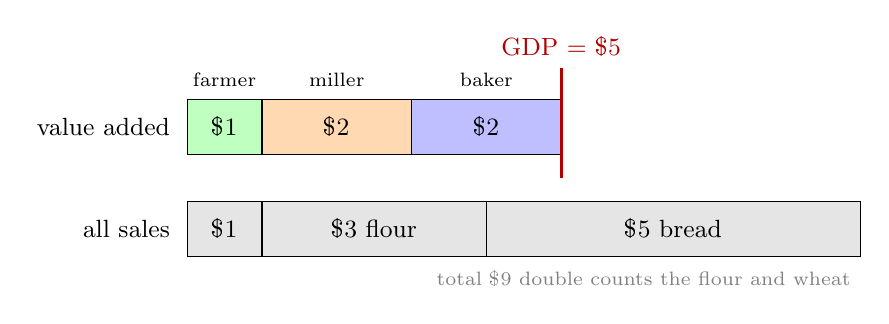
\begin{tikzpicture}[x=0.95cm, y=1cm, every node/.style={font=\small}]
  \fill[green!25] (0,1.2) rectangle (1,1.9); \draw (0,1.2) rectangle (1,1.9);
  \fill[orange!30] (1,1.2) rectangle (3,1.9); \draw (1,1.2) rectangle (3,1.9);
  \fill[blue!25] (3,1.2) rectangle (5,1.9); \draw (3,1.2) rectangle (5,1.9);
  \node at (0.5,1.55) {\$1}; \node at (2,1.55) {\$2}; \node at (4,1.55) {\$2};
  \node[font=\scriptsize] at (0.5,2.15) {farmer}; \node[font=\scriptsize] at (2,2.15) {miller}; \node[font=\scriptsize] at (4,2.15) {baker};
  \node[anchor=east] at (-0.1,1.55) {value added};
  \draw[very thick, red!70!black] (5,0.9) -- (5,2.3) node[above] {GDP $=$ \$5};
  \fill[gray!20] (0,-0.1) rectangle (9,0.6); \draw (0,-0.1) rectangle (1,0.6); \draw (1,-0.1) rectangle (4,0.6); \draw (4,-0.1) rectangle (9,0.6);
  \node at (0.5,0.25) {\$1}; \node at (2.5,0.25) {\$3 flour}; \node at (6.5,0.25) {\$5 bread};
  \node[anchor=east] at (-0.1,0.25) {all sales};
  \node[anchor=north east, text=gray, font=\scriptsize] at (9,-0.15) {total \$9 double counts the flour and wheat};
\end{tikzpicture}
\end{center}

\begin{important}[What GDP excludes]
\begin{itemize}
  \item Purchases of \emph{used} goods (produced in an earlier period).
  \item Purchases of \emph{financial assets} (stocks, bonds): these are transfers of
        ownership, not production. (A broker's commission is a service and does count.)
  \item Government \emph{transfer payments} (EI benefits, CPP payments), since nothing is
        produced in exchange.
  \item Intermediate goods (to avoid double counting).
\end{itemize}
\end{important}

\section{GDP and the circular flow of expenditure and income}

GDP measures the value of production, which also equals total expenditure on final goods
and services and total income.

\begin{center}
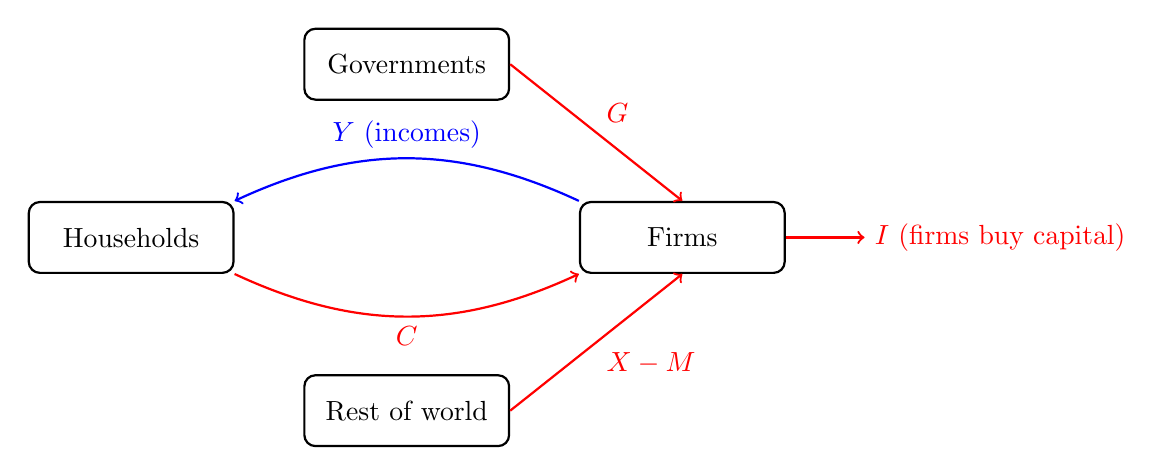
\begin{tikzpicture}[box/.style={draw, thick, rounded corners, minimum width=2.6cm, minimum height=0.9cm}]
  \node[box] (H) at (0,0) {Households};
  \node[box] (F) at (7,0) {Firms};
  \node[box] (G) at (3.5,2.2) {Governments};
  \node[box] (R) at (3.5,-2.2) {Rest of world};
  \draw[->, thick, blue] (F.north west) to[bend right=25] node[above] {$Y$ (incomes)} (H.north east);
  \draw[->, thick, red] (H.south east) to[bend right=25] node[below] {$C$} (F.south west);
  \draw[->, thick, red] (G.east) -- node[above right] {$G$} (F.north);
  \draw[->, thick, red] (R.east) -- node[below right] {$X - M$} (F.south);
  \draw[->, thick, red] (F.east) -- ++(1,0) node[right] {$I$ (firms buy capital)};
\end{tikzpicture}
\end{center}

\subsection{Households and firms}

Households sell, and firms buy, the services of labour, capital, land and
entrepreneurship in \emph{factor markets}. For these services firms pay income to
households:
\[
  \text{Total income } (Y) = \text{wages} + \text{interest} + \text{rent} + \text{profit}.
\]
Firms sell, and households buy, consumer goods and services in \emph{goods markets}.
Total payment for these is \emph{consumption expenditure} ($C$). Firms also buy new
plant, equipment and buildings and add to their inventories; these purchases are
\emph{investment} ($I$). Retained profits and household saving, channelled through
financial markets, finance investment.

\subsection{Governments}

Governments buy goods and services from firms; this is \emph{government expenditure on
goods and services} ($G$). Governments finance it with taxes. Taxes, subsidies and
\emph{transfer payments} (such as EI benefits) redistribute income, but they are not
expenditure on goods and services and are not part of $G$.

\subsection{Rest of the world}

Canadian firms sell goods and services to the rest of the world (\emph{exports}, $X$)
and Canadians buy goods and services produced abroad (\emph{imports}, $M$).
\[
  \text{Net exports} = X - M,
\]
which is positive when Canada exports more than it imports and negative otherwise.

\subsection{GDP equals expenditure equals income}

Total expenditure on goods and services produced in Canada equals
\[
  Y = C + I + G + X - M.
\]
Firms pay out everything they receive as incomes (wages, interest, rent, and profit is
whatever is left), so aggregate income equals aggregate expenditure, and both equal the
value of production:
\[
  \boxed{\text{GDP} = C + I + G + X - M = \text{aggregate income}.}
\]

\section{Why is it ``gross''?}

``Gross'' means \emph{before} deducting the depreciation of capital; the opposite of gross
is \emph{net}.

\begin{definition}[Depreciation, gross and net investment]
\emph{Depreciation} is the decrease in the value of a firm's capital that results from
wear and tear and obsolescence. \emph{Gross investment} is the total amount spent on new
capital and on replacing depreciated capital. \emph{Net investment} is the change in the
value of capital:
\[
  \text{Net investment} = \text{gross investment} - \text{depreciation}.
\]
\end{definition}

GDP uses gross investment, so it includes the production of capital that merely replaces
worn-out capital. Net domestic product (at factor cost) $=$ GDP $-$ depreciation (and
adjusting for indirect taxes, below).

\section{Measuring Canada's GDP}

Statistics Canada measures GDP in the \emph{National Income and Expenditure Accounts}
using two approaches.

\subsection{The expenditure approach}

Add up the four components of expenditure: $C + I + G + (X - M)$. In Canada, consumption
is roughly 55--58\% of GDP, investment about 20--23\%, government about 25\%, and net
exports are small (positive or negative) even though exports and imports are each about
30\% of GDP.

\subsection{The income approach}

Add up the incomes paid to factors of production. Statistics Canada groups them as
\begin{enumerate}
  \item wages, salaries and supplementary labour income (compensation of employees); and
  \item other factor incomes (corporate profits, interest and investment income, farmers'
        and unincorporated business income).
\end{enumerate}
The sum is \emph{net domestic product at factor cost}. Two adjustments convert it to GDP:
\begin{itemize}
  \item Add \emph{indirect taxes less subsidies} (e.g.\ GST/HST). Market prices include
        sales taxes and exclude subsidies, so factor cost understates market value.
  \item Add \emph{depreciation} (capital consumption allowances), because factor incomes
        are measured net of depreciation.
\end{itemize}
Any remaining gap between the two approaches is the \emph{statistical discrepancy}.

\begin{example}[Both approaches]
An economy (billions of dollars) has $C = 1200$, $I = 400$, $G = 500$, $X = 600$,
$M = 550$. Expenditure approach:
\[
  \text{GDP} = 1200 + 400 + 500 + (600 - 550) = 2150.
\]
On the income side: wages and other labour income 1150, other factor incomes 560,
indirect taxes less subsidies 240, depreciation 200. Then
\[
  \underbrace{1150 + 560}_{\text{NDP at factor cost} = 1710} + 240 + 200 = 2150,
\]
matching the expenditure approach, with no statistical discrepancy.
\end{example}

\begin{center}
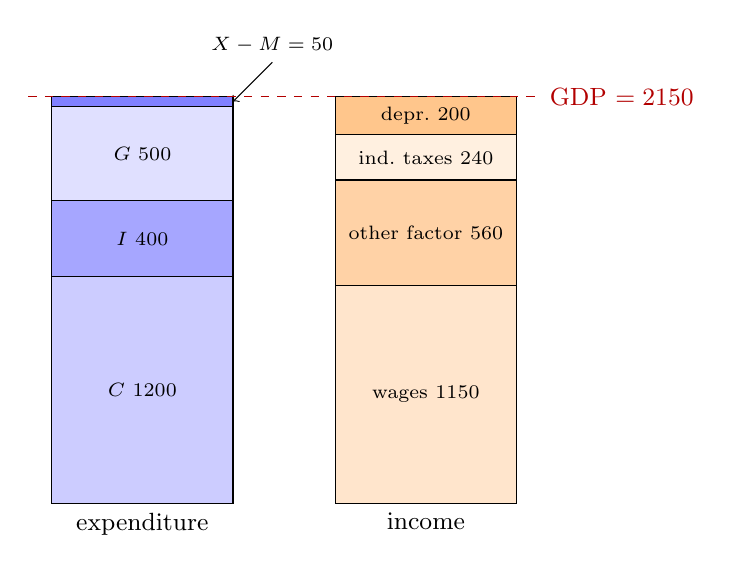
\begin{tikzpicture}[every node/.style={font=\small}]
  \fill[blue!20] (0,0.000) rectangle (2.3,2.880); \draw (0,0.000) rectangle (2.3,2.880);
  \node[font=\scriptsize] at (1.15,1.440) {$C$ 1200};
  \fill[blue!35] (0,2.880) rectangle (2.3,3.840); \draw (0,2.880) rectangle (2.3,3.840);
  \node[font=\scriptsize] at (1.15,3.360) {$I$ 400};
  \fill[blue!12] (0,3.840) rectangle (2.3,5.040); \draw (0,3.840) rectangle (2.3,5.040);
  \node[font=\scriptsize] at (1.15,4.440) {$G$ 500};
  \fill[blue!50] (0,5.040) rectangle (2.3,5.160); \draw (0,5.040) rectangle (2.3,5.160);
  \node[font=\scriptsize] at (1.15,5.100) {};
  \node[below] at (1.15,0) {expenditure};
  \fill[orange!20] (3.6,0.000) rectangle (5.9,2.760); \draw (3.6,0.000) rectangle (5.9,2.760);
  \node[font=\scriptsize] at (4.75,1.380) {wages 1150};
  \fill[orange!35] (3.6,2.760) rectangle (5.9,4.104); \draw (3.6,2.760) rectangle (5.9,4.104);
  \node[font=\scriptsize] at (4.75,3.432) {other factor 560};
  \fill[orange!12] (3.6,4.104) rectangle (5.9,4.680); \draw (3.6,4.104) rectangle (5.9,4.680);
  \node[font=\scriptsize] at (4.75,4.392) {ind.\ taxes 240};
  \fill[orange!45] (3.6,4.680) rectangle (5.9,5.160); \draw (3.6,4.680) rectangle (5.9,5.160);
  \node[font=\scriptsize] at (4.75,4.920) {depr.\ 200};
  \node[below] at (4.75,0) {income};
  \draw[<-] (2.3,5.100) -- (2.8,5.6) node[above, font=\scriptsize] {$X - M = 50$};
  \draw[dashed, red!70!black] (-0.3,5.160) -- (6.2,5.160) node[right] {GDP $= 2150$};
\end{tikzpicture}
\end{center}

\section{Nominal GDP and real GDP}

\begin{definition}[Real and nominal GDP]
\emph{Nominal GDP} is the value of final goods and services produced in a given year
valued at the prices that prevailed in that \emph{same} year. \emph{Real GDP} is the
value of final goods and services produced in a given year when valued at the prices of a
\emph{reference base year}.
\end{definition}

Nominal GDP can rise because production rises or because prices rise; real GDP removes
the effect of price changes, so it measures changes in the quantity of production.

\begin{definition}[GDP deflator]
\[
  \text{GDP deflator} = \frac{\text{nominal GDP}}{\text{real GDP}} \times 100.
\]
In the base year nominal and real GDP are equal, so the deflator is 100.
\end{definition}

\begin{example}[Real GDP and the deflator]
An economy produces only apples and pens. Base year 2015:
\begin{center}
\begin{tabular}{lcccc}
\toprule
 & \multicolumn{2}{c}{2015 (base)} & \multicolumn{2}{c}{2016} \\
 & Quantity & Price & Quantity & Price \\
\midrule
Apples & 100 & \$1.00 & 110 & \$1.20 \\
Pens & 50 & \$2.00 & 60 & \$2.50 \\
\bottomrule
\end{tabular}
\end{center}
\begin{itemize}
  \item Nominal GDP 2015 $= 100(1) + 50(2) = \$200$ $=$ real GDP 2015.
  \item Nominal GDP 2016 $= 110(1.20) + 60(2.50) = 132 + 150 = \$282$.
  \item Real GDP 2016 (2015 prices) $= 110(1) + 60(2) = 110 + 120 = \$230$.
  \item GDP deflator 2016 $= 282/230 \times 100 \approx 122.6$.
  \item Real GDP growth $= (230 - 200)/200 \times 100 = 15\%$, while nominal GDP grew
        $(282 - 200)/200 \times 100 = 41\%$. Most of the nominal growth was price
        increases (prices rose about 22.6\%).
\end{itemize}
\end{example}

\begin{remark}[Chained-dollar real GDP]
Statistics Canada actually uses the \emph{chain-weighted} (Fisher) method: it computes
real growth each year using the average of the growth rates at the previous year's and
the current year's prices, then links (chains) these growth rates back to the reference
year. Results are reported as ``chained 2012 dollars'' (the reference year has changed
over time, e.g.\ 2007 and 2012). The idea is the same as the base-year method but avoids
outdated price weights.
\end{remark}

\section{The uses and limitations of real GDP}

\subsection{Standard of living over time}

\begin{definition}[Real GDP per person]
\[
  \text{real GDP per person} = \frac{\text{real GDP}}{\text{population}}.
\]
\end{definition}

The growth rate of a variable from year $t-1$ to year $t$ is
\[
  \text{growth rate} = \frac{X_t - X_{t-1}}{X_{t-1}} \times 100,
\]
and approximately,
\[
  \text{growth of real GDP per person} \approx \text{growth of real GDP} -
  \text{growth of population}.
\]

\begin{example}
Real GDP rises from \$1{,}800 billion to \$1{,}854 billion while population rises from
36.0 million to 36.36 million. Real GDP grew $54/1800 = 3\%$, population grew
$0.36/36 = 1\%$. Real GDP per person went from \$50{,}000 to
$1{,}854{,}000/36.36 \approx \$50{,}990$, growth $\approx 1.98\%$, close to $3\% - 1\% = 2\%$.
\end{example}

\begin{important}[Rule of 70]
The number of years it takes a variable growing at $g\%$ per year to double is about
$70/g$. At 2\% per year real GDP per person doubles in about 35 years; at 7\% in about
10 years. Small differences in growth rates compound into huge differences in living
standards.
\end{important}

\begin{center}
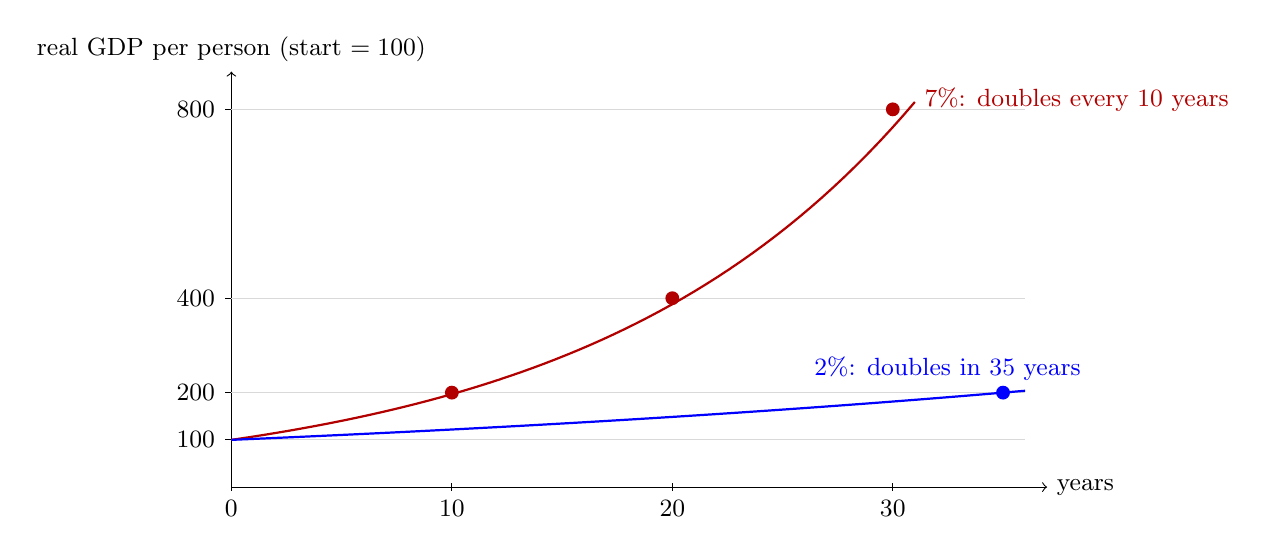
\begin{tikzpicture}[x=0.28cm, y=0.006cm, every node/.style={font=\small}]
  \draw[->] (0,0) -- (37,0) node[right] {years};
  \draw[->] (0,0) -- (0,880) node[above] {real GDP per person (start $= 100$)};
  \foreach \t in {0,10,20,30} \draw (\t,8) -- (\t,-8) node[below] {\t};
  \foreach \v in {100,200,400,800} { \draw (0.3,\v) -- (-0.3,\v) node[left] {\v}; \draw[gray!30] (0,\v) -- (36,\v); }
  \draw[thick, red!70!black, domain=0:31, samples=60] plot (\x, {100*exp(0.0677*\x)});
  \draw[thick, blue, domain=0:36, samples=60] plot (\x, {100*exp(0.0198*\x)});
  \node[red!70!black, anchor=west] at (31,820) {$7\%$: doubles every $10$ years};
  \node[blue, anchor=west] at (26,250) {$2\%$: doubles in $35$ years};
  \foreach \t/\v in {10/200, 20/400, 30/800} \fill[red!70!black] (\t,\v) circle (2.5pt);
  \fill[blue] (35,200) circle (2.5pt);
\end{tikzpicture}
\end{center}

\begin{definition}[Potential GDP and the business cycle]
\emph{Potential GDP} is the value of real GDP when all the economy's factors of
production are fully employed. The \emph{business cycle} is the periodic but irregular
up-and-down movement of total production and other measures of economic activity. Its
phases are \emph{expansion} and \emph{recession} (in Canada, commonly a decrease in real
GDP for at least two successive quarters), and its turning points are the \emph{peak} and
the \emph{trough}.
\end{definition}

\begin{center}
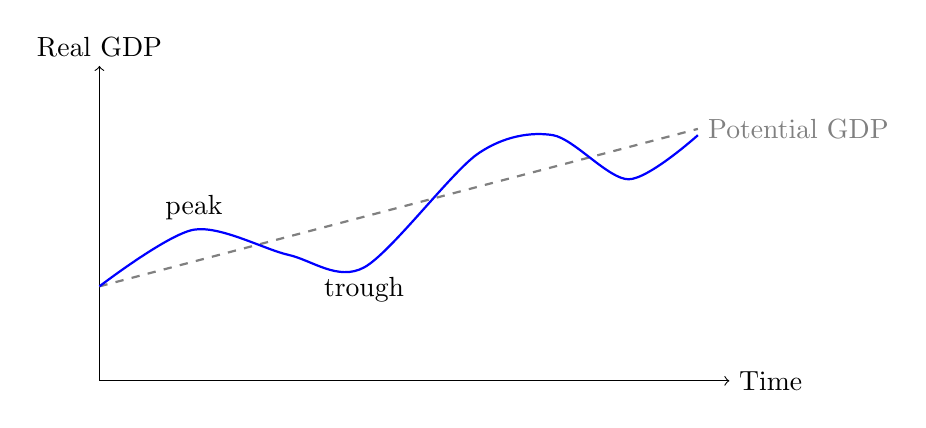
\begin{tikzpicture}[scale=0.8]
  \draw[->] (0,0) -- (10,0) node[right] {Time};
  \draw[->] (0,0) -- (0,5) node[above] {Real GDP};
  \draw[thick, dashed, gray] (0,1.5) -- (9.5,4) node[right] {Potential GDP};
  \draw[thick, blue] plot[smooth] coordinates {(0,1.5) (1.5,2.4) (3,2.0) (4.2,1.8) (6,3.6) (7.2,3.9) (8.4,3.2) (9.5,3.9)};
  \node[above] at (1.5,2.4) {peak};
  \node[below] at (4.2,1.8) {trough};
\end{tikzpicture}
\end{center}

\subsection{Comparing living standards across countries}

To compare real GDP across countries we must value output in the same prices.
International comparisons use \emph{purchasing power parity} (PPP) prices, which value
goods at the same prices in every country. Using market exchange rates understates the
real GDP of poorer countries, where non-traded services are cheap.

\subsection{Limitations of real GDP}

Real GDP is a measure of production, not of well-being. It omits:
\begin{itemize}
  \item \textbf{Household production}: cooking, cleaning, child care done at home.
  \item \textbf{Underground economic activity}: illegal activity and unreported legal
        activity (cash jobs to avoid taxes).
  \item \textbf{Leisure time}: more leisure raises well-being but not GDP.
  \item \textbf{Environmental quality}: pollution and resource depletion are not
        subtracted.
  \item \textbf{Health and life expectancy}, \textbf{political freedom and social
        justice}.
\end{itemize}
Broader measures include the UN's Human Development Index (HDI), which combines income,
health and education.

\section{Summary}

\begin{itemize}
  \item GDP: market value of final goods and services produced within a country in a
        period. Count final goods only (or sum value added).
  \item Circular flow: $Y = C + I + G + X - M$; production $=$ expenditure $=$ income.
  \item Gross includes depreciation; net investment $=$ gross investment $-$
        depreciation.
  \item Statistics Canada uses the expenditure approach and the income approach; the
        income approach adds indirect taxes less subsidies and depreciation to factor
        incomes.
  \item Real GDP values output at base-year (or chained) prices; GDP deflator $=$
        nominal/real $\times 100$.
  \item Real GDP per person measures living standards over time; rule of 70; the business
        cycle fluctuates around potential GDP. GDP leaves out household production, the
        underground economy, leisure and environmental quality.
\end{itemize}
